\documentclass[legalpaper]{article}
\title{\vspace{-4cm}CS3104 Practical Week 7}
\author{170025298}
\date{}

\usepackage{graphicx}
\usepackage{float}
\usepackage[utf8]{inputenc}
\usepackage[font = {small,it}]{caption}
\graphicspath{{images/}}

\usepackage[margin=1.2in]{geometry}

\pagenumbering{arabic}

\begin{document}
	\maketitle
	\section{Design}
	There is a picture basically can describe my description. The method I chose is to design an inode which includes basically file control block implementation and 13 direct access pointer, 1 single indirect pointer, 1 double indirect pointer, and one triple indirect pointer.\par
	\begin{figure}[H]
	\centering
	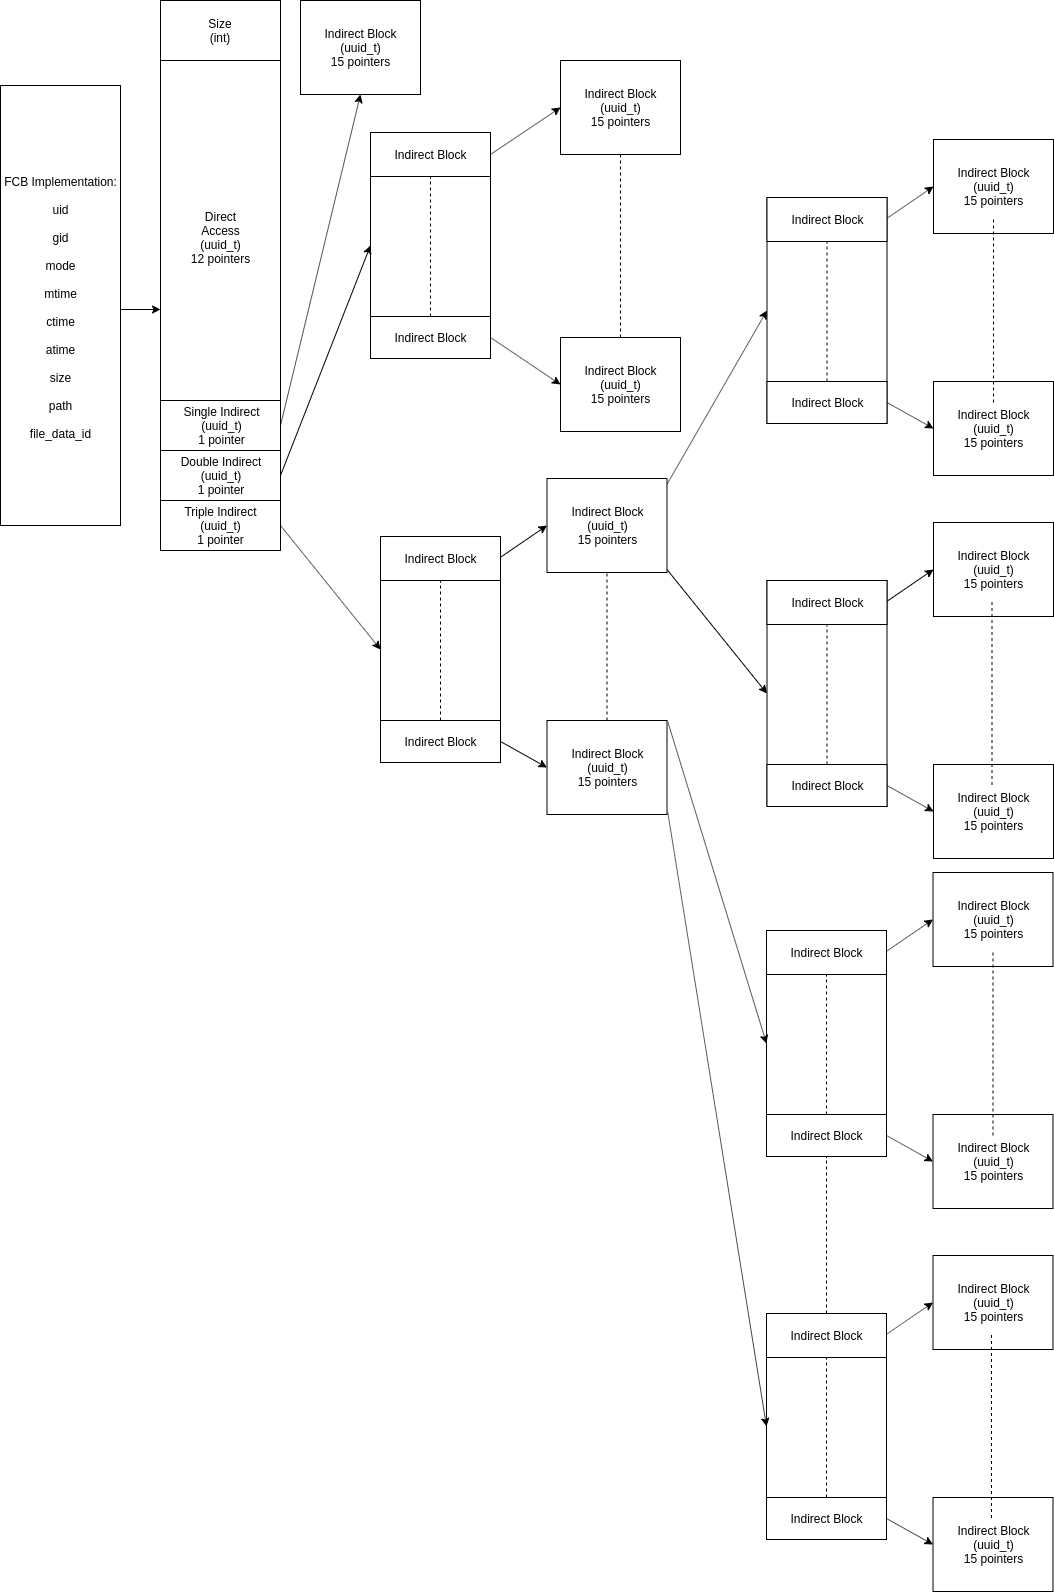
\includegraphics[width = \textwidth]{inode}
	\caption{Inode full design}
	\end{figure}
	There is a root inode in the memory with a simple and understandable key that can access the inode. For an arbitrary length file path and smaller memory use, we created a structure which mainly contains the key of the fcb and the name of the file.  This structure can be called entry, which is the entry of the fcb.\par
	For directories, entries will connect to the direct access pointer first. Only when the direct access pointer used up, it will generate a UUID and connect to the indirect pointers. Each indirect block has 15 pointers for connecting to different access blocks. So the single indirect entries will allow 15 entries, double indirect entries allow $15^{15}$ entries and triple indirect entries allow $15^{15^{15}}$ entries, which is actually big enough for storing all kinds of things.\par
	Detailed design is shown as follows:\par
	\begin{figure}[H]
	\centering
	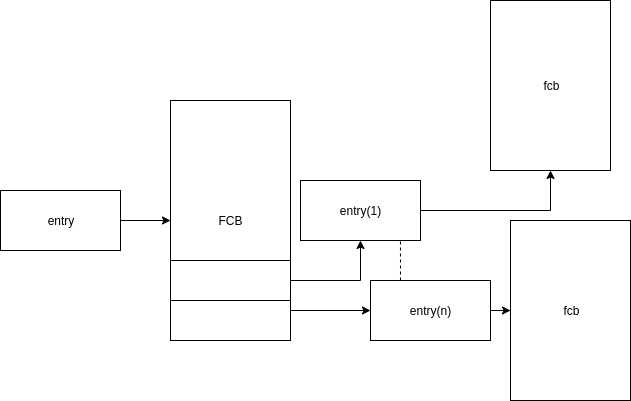
\includegraphics[width = \textwidth]{addnode}
	\caption{design}
	\end{figure}
	FCB only pay response to other entries but does not care about any other fcb. In a contract, entries only pay response to its FCB but do not pay attention to another entries. This makes finding a specific file much easier and make the file structure more clear, as each entry has a single pathname and a single UUID key, which has an obvious advantage on implementing a file system.
	\section{Implementation}
	In this section, I will take an example path to explain the implementation: $/a/aa/aaaa.txt$
	\subsection*{get attribute}
	This function will judge whether it is root file first, then if not it will directly access the fcb of the path and retrieve the information of such block. 
	\subsection*{access to the path from local argument}
	This can be finished by using $strtok(str, "/")$, each strtok will change one $/$ to $\backslash 0$ and return the pointer to the string, which is a terminate of the string. This allows hierarchy access and to the next file control block. An example of this is when we use strtok to solve the path, we will get $a$ the first time, then we got $aa$ and so on.
	\subsection*{splitting path name and dir name}
	This can be done by using $strrchr()$, which allows programmers to find last delimit and return the pointer of such delimit. Then I replaced the pointer to $\backslash 0$ and the path starts with starting pointer and the file name is the value of $pointer + 1$
	\subsection*{create file and directories}
	These two functions can be done just the same, we will access to the path by using splitting function and access function, then the program will find a space to generate a new UUID and then call the create function and write back new fcb and old fcb.
	\subsection*{find specific fcb using name}
	When we access the directory fcb, we will fetch entries with for loop and use strcmp() to compare names stored in the entrance node with the filename given. If the filename is the same as the pathname, it will return 0 and a passing pointer to fcb and entrance node in the local argument.	
	\subsection*{deletion}
	When we want to delete a file, the program will access the path first, such as when deleting $aaaa.txt$, the program will access $/a/aa$. Then the program will access the fcb and swipe data in direct access blocks, and then delete data from unqlite. Then it will delete the entrance node and fcb node from the unqlite and clear the key in the fcb of the path. Then write back will happen and deletion has completed.
	\subsection*{free space generator}
	When we are making directories or writing files, we will need free space for storing the file or directory UUID. A generator will read through direct access and then find a zero UUID. Then the program will generate this UUID and write back the data block. Such UUID will be passed outside the function for storing the data block. 
	\subsection*{modular}
	It is quite complex and lots of duplicates when trying to fetch and store the data block. So I make things modular such as to define functions of reading and fetching, which actually prevented lots of duplicates.
	\subsection*{writing to the file}
	Writing to the file will create a file structure first, then create the entry fcb pair if it does not exist. The file structure will link to the first fcb direct access and the fcb should be write back with modification. 
	\subsection*{write log}
	Write log can be regarded as panic in go. It will write which part goes wrong and error will return from each functions. If it succeed, only working log will be returned.
	\section{Testing}
	\subsection*{chmod and chown(Figure 3)}
	Chmod and Chown will change the accessible protection mode of the file.
	\begin{figure}[H]
	\centering
	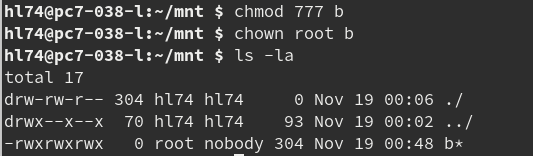
\includegraphics[width = \textwidth]{ch}
	\caption{chmod and chown}
	\end{figure}
	\subsection*{hierarchy system(Figure 4)}
	Hierarchy system will shows the system with tree structure
	\begin{figure}[H]
	\centering
	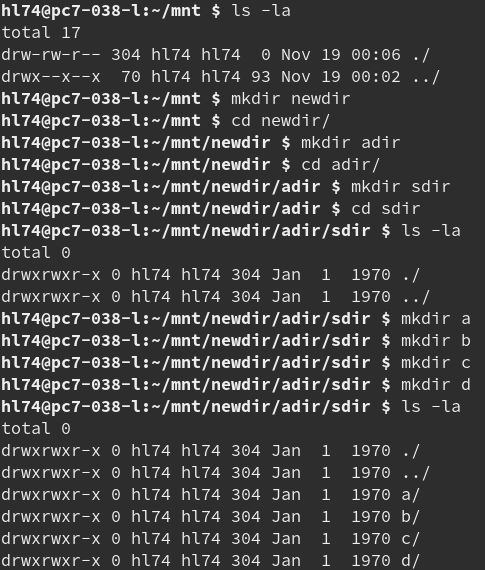
\includegraphics[width = \textwidth]{hier}
	\caption{make directory inside another directory}
	\end{figure}
	\subsection*{utime(Figure 5)}
	utime allows to change modification time for file.
	\begin{figure}[H]
	\centering
	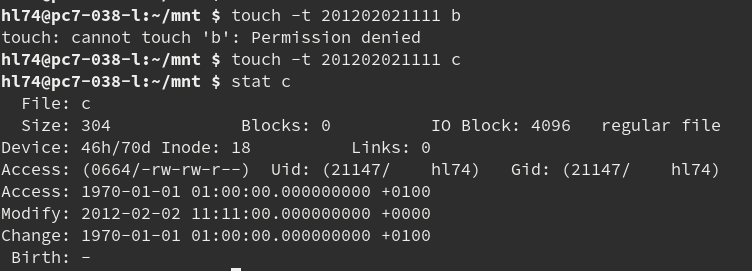
\includegraphics[width = \textwidth]{permutime}
	\caption{chmod and chown}
	\end{figure}
	\subsection*{remove directory and remove file(Figure 6)}
	rmdir and rm allows user to remove the directory and remove the file
	\begin{figure}[H]
	\centering
	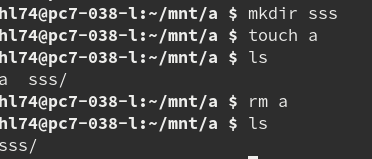
\includegraphics[width = \textwidth]{rmunlink}
	\caption{remove}
	\end{figure}
	\subsection*{Writing to a file(Figure 7)}
	using cat in a terminal allows users to read the file data. Using > allows user to write into data with pipe.
	\begin{figure}[H]
	\centering
	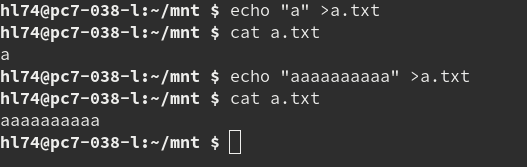
\includegraphics[width = \textwidth]{write}
	\caption{read and write}
	\end{figure}
	\section{Summary}
	Luckily, basic implementation has all done and returning message is not listed in the requirement. Several optional functions has not implemented and there are still lots of bugs available such as returning messages. The messages returned by UNQLITE is not the same as the message returned from FUSE. I am currently in my lowest expect for my final grades and feels quite upset.\\\\
	I have actually learned and practices a lot on operating on passing a pointer to the functions. Even I have not implemented all what I have designed and there is no extension that I have done, I have noticed my disadvantages on programming, which is I always regard the question more complex such as arbitrary limit, I have though a lot about it and finally I found the arbitrary limit does not means I have to store 10000+ for the file.\\\\
	Actually I am really upset these days, I have worked for 30+ hours without any sleep in Saturday, but what I achieved is just a half of basic and with full of bugs. Panic cannot solve problems, a better way to solve panic could be start my working much earlier and do as much as I can everyday.
\end{document}